\documentclass[a4paper,10pt,conference,compsocconf,final]{IEEEtran}

\usepackage[hyphens]{url}
\usepackage{hyperref}
\usepackage{color}
\usepackage[utf8]{inputenc}
\usepackage[stretch=10]{microtype} 
\usepackage{graphicx}
\usepackage{booktabs} 
\usepackage[mathscr]{eucal}
\usepackage{mathtools}
\usepackage{enumerate}
\usepackage{xspace}
\usepackage{shortvrb}
\usepackage{mdwmath} 
\usepackage{verbatim}
\usepackage{multirow}
\usepackage[square,comma,numbers,sort]{natbib}
\usepackage{balance}
\usepackage{times}
\renewcommand{\ttdefault}{cmtt}

\usepackage[tight,footnotesize]{subfigure}
\newcommand\method[1]{{\sf\small{#1}}}
\newcommand{\opstyle}[1]{\mbox{\textsc{#1}}}
\newcommand{\var}[1]{\mbox{\emph{#1}}}
\newcommand{\svar}[1]{\mbox{\small\emph{#1}}}
\newcommand{\ssvar}[1]{\mbox{\scriptsize\emph{#1}}}
\def\D{\hphantom{1}}
\def\C{\hphantom{1,}}
%-- Sizes 
\newcommand\kb[1]{$#1$\,kB}
\newcommand\mb[1]{$#1$\,MB} 
\newcommand\gb[1]{$#1$\,GB}
\newcommand\tb[1]{$#1$\,TB} 
%--- Latex hyphenation sucks, make it go away.
\hyphenpenalty=5000
\tolerance=1000

%

\newcommand{\myparagraph}[1]{\vspace*{1ex}\noindent{\textbf{#1.}}~}
\newcommand{\shane}[1]{\textrm{\textcolor{orange}{Shane says: #1}}}
\newcommand{\ruey}[1]{\textrm{\textcolor{red}{Ruey says: #1}}}
\newcommand{\joel}[1]{\textrm{\textcolor{magenta}{Joel says: #1}}}

\usepackage{todonotes}
\newcommand{\am}{\todo[author=AM, color=red!20!white,inline]}

\begin{document} % 

% paper title % can use linebreaks \\ within to get better formatting as desired 
\title{RMIT at the TREC 2016 LiveQA Track}
\author{\IEEEauthorblockN{%
Joel Mackenzie,
Ruey-Cheng Chen,
J. Shane Culpepper}
\IEEEauthorblockA{RMIT University\\
Melbourne, Australia\\ 
{\{joel.mackenzie, ruey-cheng.chen, shane.culpepper\}@rmit.edu.au}
}}

\maketitle

\begin{abstract} 
This paper describes the four systems RMIT fielded for the
{\opstyle{TREC}} 2016 LiveQA task and the associated experiments.
Similar to last year, the results show that simple solutions tend
to work best, and that our improved baseline systems achieved
an above-average performance.
We use a commercial search engine as a first stage retrieval
mechanism and compare it with our internal system which uses
a carefully curated document collection.
Somewhat surprisingly, we found that on average the small curated
collection performed better within our current framework, warranting
further studies on when and when not to use an external resource,
such as a publicly available search engine API.
Finally, we show that small improvements to performance can
substantially reduce failure rates.
\end{abstract}

\begin{IEEEkeywords} 
  \opstyle{TREC} LiveQA 2016; RMIT; paragraph retrieval; summarization; learning to rank
\end{IEEEkeywords}

\section{Overview}
\label{overview}

In the TREC LiveQA 2016 challenge, we continued to explore ideas
within an established two-stage answer-finding framework used in last
year's LiveQA challenge.
Our long-term goal is to build a fully functional, modular multi-stage
retrieval system that cascades candidate results through a series
of increasingly complex filters.
In our current system, a first-stage retrieval module is employed to
first populate a good set of answer-bearing passages, and then a
summarization module is used to generate the final answers via
passage re-ranking or query-biased summarization.

We configured four different systems following two distinct
strategies.
First, we looked at the retrieval part and made comparisons between
two common retrieval settings: retrieving passages from a home-made
question-answering test collection, and retrieving snippets from a
commercial search engine.
Second, we made comparisons between two common answer-producing
strategies: answer re-ranking using a Learning-to-Rank (LtR) model,
and query-biased summarization using a max-coverage optimization
model.
This has led us to consider the following research questions: 

\myparagraph{RQ 1:}
{\emph{ 
Which strategy produces better passages, retrieving from a local test
collection or pulling content from a commercial search engine?
}} 

\myparagraph{RQ 2:}
{\emph{
Which strategy produces better answers, locating the best passages
directly or generating a succinct summary out of the top passages?
}} 

\myparagraph{RQ 3:}
{\emph{
Does the efficiency of the first-stage retrieval module contribute to
the failure rate on longer questions?
}} 

\medskip

We also did a careful per query analysis using the 2015 queries to
determine how efficiency impacted the performance with regard to the
time budget.
We found that returning the top-$k$ paragraphs from our local
collection followed by generating the answer with the coverage-based
summarizer provided the most effective answers.

\section{Methodology}
We now describe the collection and retrieval setting used in our
system. 

\subsection{Server architecture}

The servers are built on top of the computing resources we allocated
from NecTAR,\footnote{\url{https://www.nectar.org.au}} the Australian
National Research cloud computing network.
Throughout the challenge, we use only one instance to host all of the
services.

\begin{figure}[t]
  \centering
  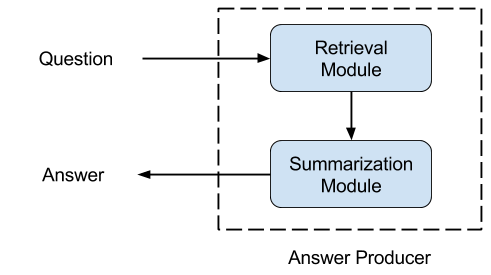
\includegraphics[width=0.8\columnwidth]{arch.png}
  \caption{System architecture for the RMIT systems.}
  \label{fig:arch}
\end{figure}

All four RMIT systems implemented a two-stage system architecture, as
illustrated in Figure~\ref{fig:arch}.
Upon receiving a question, the system would first convert it into a
bag-of-words query, and run the query through the Retrieval Module
(cf.  Section~\ref{sec:retrieval}).
The Retrieval Module retrieved a set of passages from the underlying
corpora and served them to the Summarization Module (cf.
Section~\ref{sec:sum}), which in turn produces a piece of text
that is coherent and long enough to fill the required answer size.

%\joel{Is this true anymore?}
%The three most relevant passages retrieved are then submitted to our 
%summarizer component, which outputs a predefined number of sentences ranked by
%relevance within the summarizer (see Section \ref{sec:sum}).

%In our final iteration, we wanted to see if a subset of ``important''
%terms derived from a headword expansion would improve performance.
%In this iteration, we extracted key terms from the original question,
%which were then trimmed.
%Query expansion of the headwords was carried out using {\method{word2vec}}.
%The reduced query with {\method{word2vec}} headword expansion is
%passed to the query processor.
%The retrieved documents were then summarized by the summarizer, and
%the first sentence is then returned as the response.

The various modules were connected using a resource allocator called
{\small{\sf Answer Producer}}, and written in the Go Programming Language.
It included graceful handling of timeouts, and guaranteed responses
within the 60 second
window.\footnote{\url{https://github.com/TimothyJones/trec-liveqa-server}}

\subsection{Run descriptions}
\label{sec:runs}

% \begin{table}[t]
%   \centering
%   \caption{A brief summary of the run settings}
%   \begin{tabular}{lll}
%     \toprule
%     & \bf Retrieval Module & \bf Summarization Module \\
%     \midrule
%     RMIT-1 & Local data + WAND index & Learning-to-Rank \\
%     RMIT-2 & Bing Search API snippets & Learning-to-Rank \\
%     RMIT-11 & Local data + WAND index & Optimization \\
%     RMIT-12 & Bing Search API snippets & Optimization \\
%     \bottomrule
%   \end{tabular}
% \end{table}

\begin{table*}[!t]
\centering
\caption{Summary of collections indexed to answer questions.\label{tbl:col}}
\begin{tabular}{p{35mm}rrl}
\toprule
{\bf Collection} & {\bf \# Paragraphs} & {\bf \# Words} & {\bf Description} \\
\midrule
% AQUAINT & $\D1{,}034$K & $\C506$M & Newswire, 1999 - 2000 \\
% AQUAINT2 & $\D\C907$K & $\C410$M & Newswire, Oct 2004 - Mar 2006 \\
Wikipedia-EN & $47{,}193$K & $1{,}775$M & Online knowledge base \\
Yahoo! Answers CQA v1.0 & $31{,}972$K & $1{,}462$M & Answers items from the Yahoo! Answers website. \\
TREC 2015 LiveQA Data & $22$K & $1.8$M & \\
\bottomrule
\end{tabular}
\end{table*}

\noindent\textbf{RMIT-1 (automatic): } A WAND bag-of-words passage
retrieval using all of the terms in the question title, with answers
generated from top-$k$ passages by using a Learning-to-Rank model.
See Section~\ref{sec:ltr} for a full description of our
Learning-to-Rank model.

\medskip

\noindent\textbf{RMIT-2 (automatic): } Bing Search API snippets using
all of the terms in the question title, with answers generated from
top-$k$ passages by using a Learning-to-Rank model.

\medskip

\noindent\textbf{RMIT-11 (automatic): } A WAND bag-of-words passage
retrieval using all of the terms in the question title, with answers
generated from top-$k$ passages by using a coverage-based
summarization algorithm.
See Section~\ref{sec:opt} for details on the summarization model.

\medskip

\noindent\textbf{RMIT-12 (automatic): } Bing Search API snippets
using all of the terms in the question title, with answers generated
from top-$k$ passages by using an optimization-based summarization
algorithm.

\medskip

\section{Retrieval Module}\label{sec:retrieval}

\subsection{Passage Retrieval Using WAND Indexes}\label{sec:wand}
\begin{figure}[t]
\centering
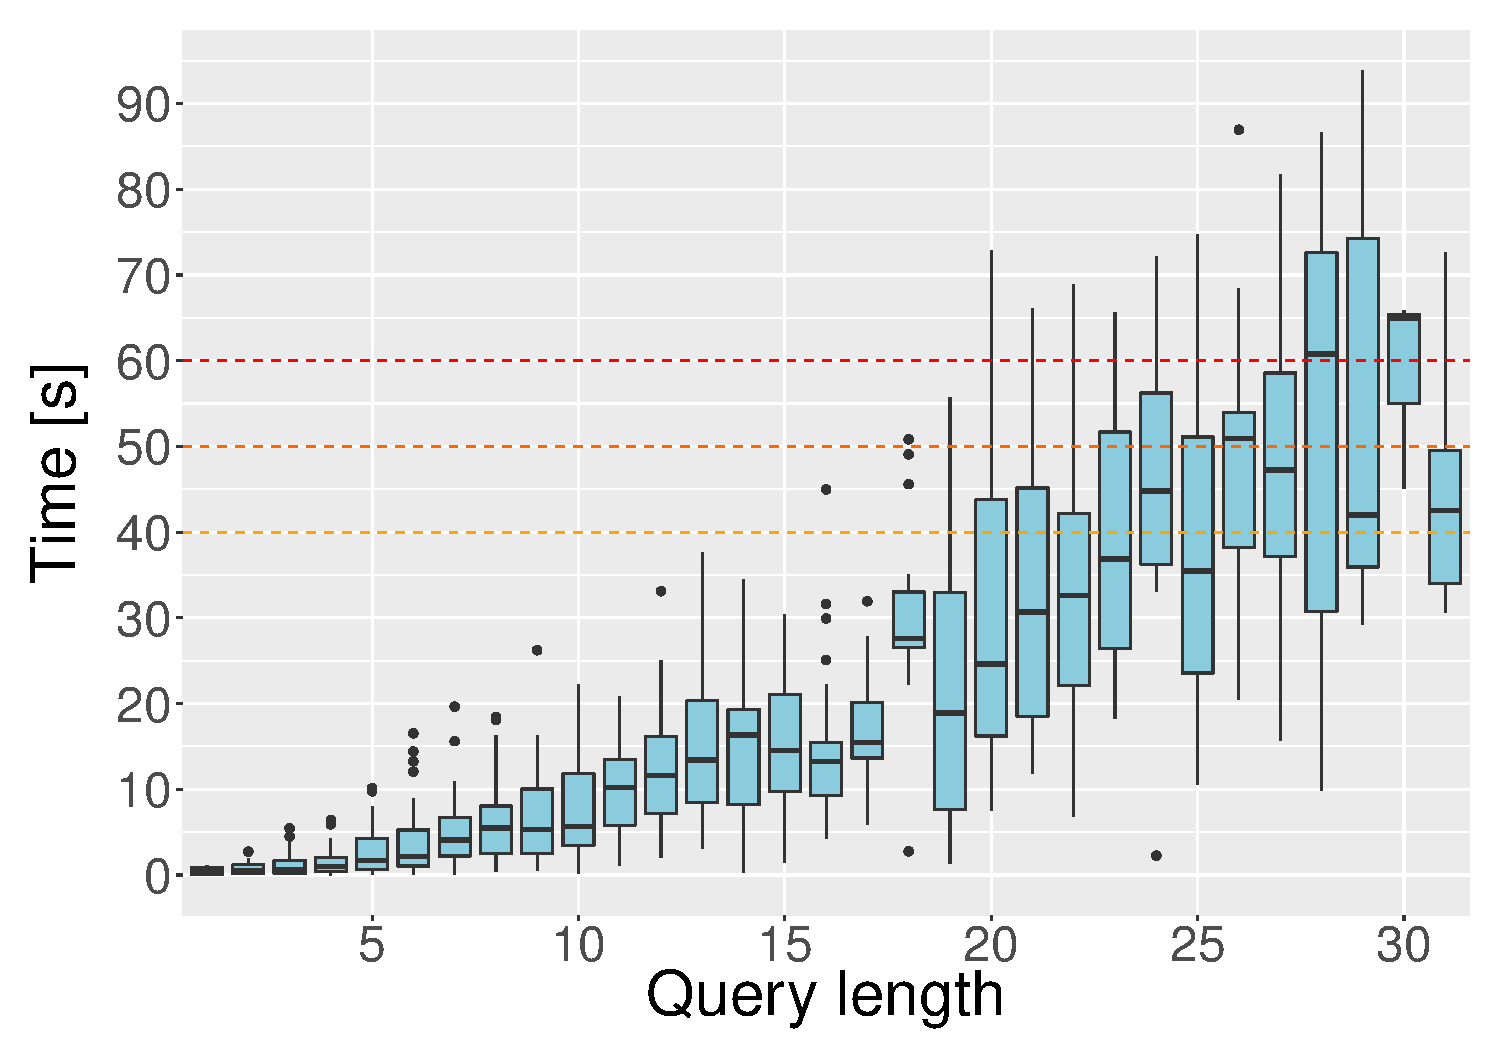
\includegraphics[width=0.45\textwidth]{indri-passage.pdf}
\caption{Query times across our test set of queries, timing the Indri
passage retrieval function,
{\texttt{\#combine[passage100:50](\ldots)}}.
The horizontal lines at 40, 50 and 60 seconds denote an increasing
chance of failure, as the retrieval budget becomes too high.
Clearly, any query above the 60s line was a failure, and any above
the 50s line was likely a failure, given the time required to
generate an answer from the candidates and return the answer to the
LiveQA server.}
\label{fig:indri-passage}
\end{figure}


\begin{figure}[t]
\centering
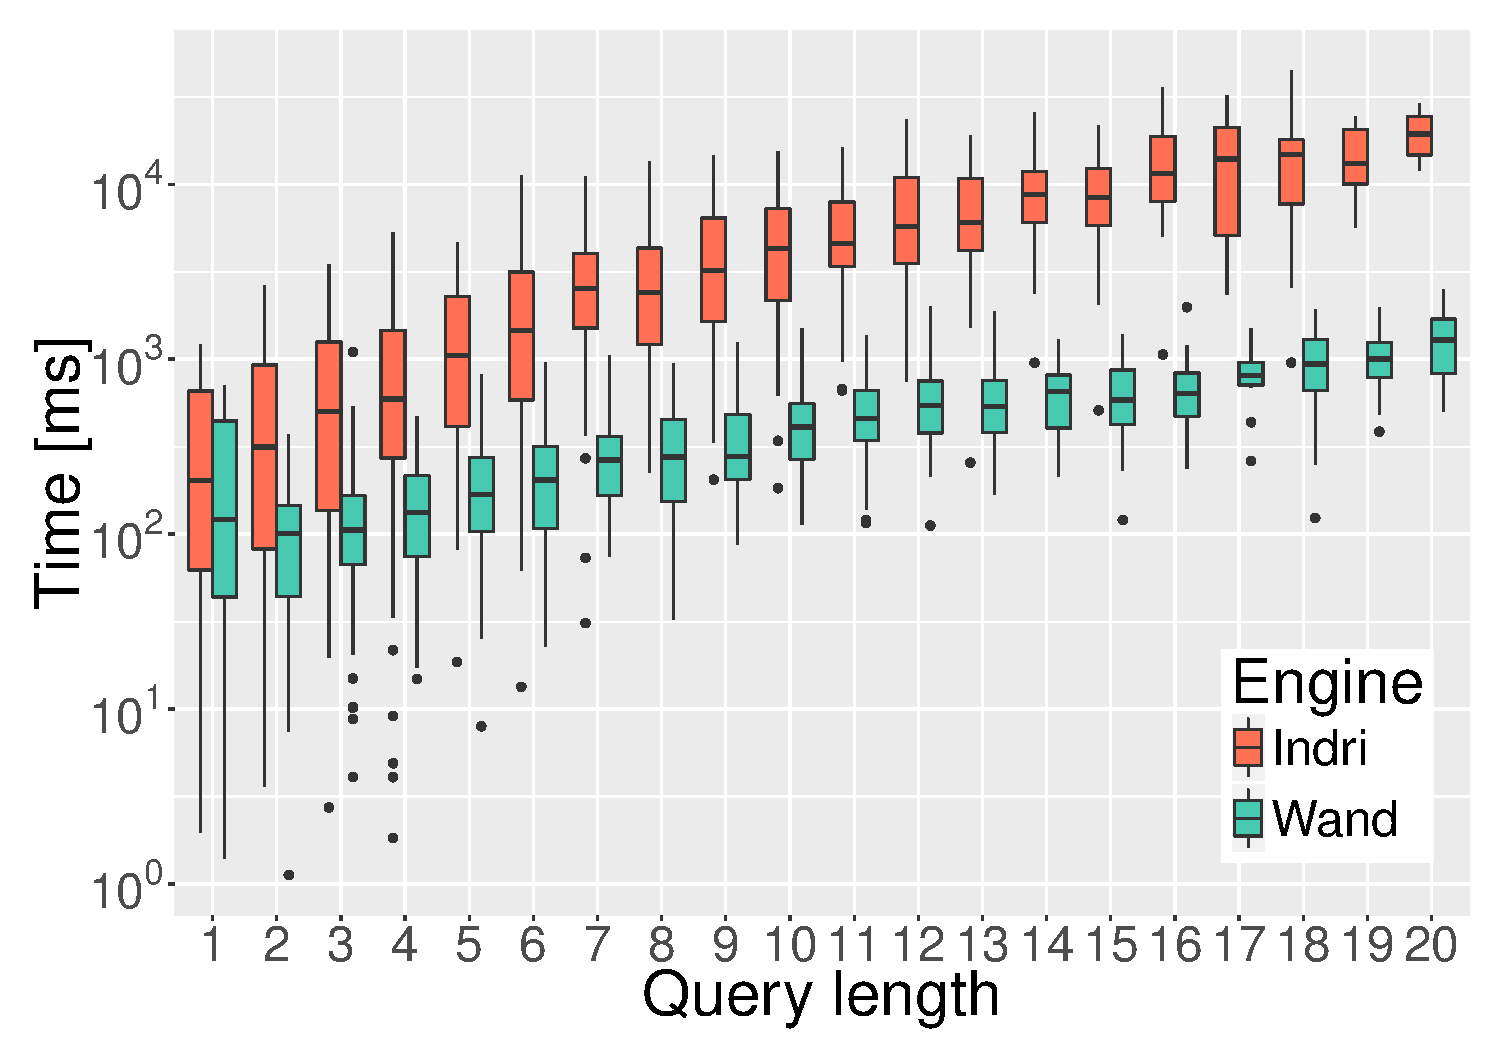
\includegraphics[width=0.45\textwidth]{timing.pdf}
\caption{Query times across our test set of queries, comparing Indri
to our WAND algorithm.
These timings are for top-$1000$ paragraph retrieval, using the bag-of-words 
BM25 ranking function. Note that time is in log scale msec, while 
Figure~{\ref{fig:indri-passage}} on the left is in seconds without a log scale.}
\label{fig:timing}
\end{figure}

%\shane{Can we add some of our earlier graphs where we compared our
%Indri performance last year relative to the new version? We had some
%interesting graphs that suggested some of our queries last year might
%have failed since the queries too a long time to run.}
%\joel{Done - Added graph for combine passage query}
% \ruey{paragraph issues addressed.}

Our first retrieval module was built on top of several
question-answering test collections, including English Wikipedia,
Yahoo!  Answers CQA data 1.0, and the TREC 2015 LiveQA dataset.
Table~{\ref{tbl:col}} shows the details for each of these test collections.
To prepare the test collection for English Wikipedia, open-source
tools such as
{\method{wp-download}}\footnote{\url{https://github.com/babilen/wp-download}}
and
{\method{wikiextractor}}\footnote{\url{https://github.com/attardi/wikiextractor}}
were used to fetch a recent dump and extract the XML contents.
Paragraphs extracted from the output of {\method{wikiextractor}} were
assigned a unique docno and got indexed using
Indri.\footnote{\url{http://www.lemurproject.org/indri/php}} For the
Yahoo!  Answers CQA data, we stripped all answer items (not just the best
answers) from the data and indexed them as documents.
No further paragraph separation was done to these answer items as
most of them were short.
No other subject/content information was incorporated (i.e.,
question title or description).
The TREC 2015 LiveQA data was prepared and indexed in a similar
fashion, with answer items treated as standalone paragraphs.

The approach taken here was similar to what we did last year
{\cite{rmit_liveqa_2015}}, but with a few subtle differences: 
Instead of using the Indri index to answer queries directly, and
utilizing the passage retrieval operator
{\texttt{\#combine[passage100:50](\ldots)}} to return a set of
candidate passages from these documents, we chose to index paragraphs
and passages directly, and using our own search system 
{\footnote{\url{https://github.com/jsc/WANDbl}}} to perform the
top-$k$ retrieval.
This allows us to use standard bag-of-words retrieval models to get a
reasonable candidate set of passages more efficiently, which can then
be passed onto the next stage of our system.
This was motivated by the scalability of Indri passage retrieval: It
does not scale well as query length increases
(Figure~\ref{fig:indri-passage}).
Given that there is a fixed time budget in the task, and queries can
be long, our new approach allows us to more reliably retrieve a set
of candidate documents within the time budget.

Our custom indexing system ({\footnotesize{\sf WANDbl}}) is a faithful
re-implementation of WAND~\citep{wand} with several engineering
performance enhancements that maximize efficiency
~{\citep{pcm13-adcs,pmc14-sigir,mcc15-adcs}}.
The index required for our system is generated from the Indri index,
and we used Krovetz stemming and the default InQuery
stoplist\footnote{\url{http://www.lemurproject.org/indri.php}}.
This yielded a single \gb{5.6} index that contained $79.2$ million
paragraphs and $15.5$ million unique terms.
The average length of an indexed paragraph was $47.4$ terms.
We use BM25 to rank the candidate passages, with the parameter
configuration of $k_1=0.9$ and $b=0.4$.\footnote{The values for $b$
and $k_1$ are different than the defaults reported by
~{\citet{rwj+94-trec}}.
These parameter choices were reported for Atire and Lucene in the
2015 IR-Reproducibility Challenge, see
{\url{github.com/lintool/IR-Reproducibility}} for further details.}

% According to our prior tests over the live stream, the question title
% contains $10$ terms on average, and the body size is around $30$ terms.
% However, as some of the question bodies can be quite long, we decided
% to construct queries using only the title.
% In two of our submitted runs, we tried different ways of expressing
% the same query intent by doing query reduction and expansion.

\begin{table}[!t]
\centering
\caption{
Comparing Title-only to Title + Description first-stage bag-of-words queries.
We report Recall@$k$, and ERR@$20$. Note that all of the Title-only 
results were found to be significantly better with a $p < 0.01$,
using a two-tailed paired $t$-test.}
\label{tab:titlevsfull}
\begin{tabular}{lcc}
\toprule
{\bf Metric} & {\bf Title-only} & {\bf Title + Description}\\
\midrule
\multicolumn{3}{c}{4+ Relevance}\\
\midrule
Recall@10   & 0.1268 & 0.0995\\
Recall@100  & 0.1870 & 0.1518\\
Recall@1000 & 0.2485 & 0.2036\\
\midrule
\multicolumn{3}{c}{3+ Relevance}\\
\midrule
Recall@10   & 0.2134 & 0.1606\\
Recall@100  & 0.3108 & 0.2457\\
Recall@1000 & 0.4129 & 0.3277\\
\midrule
\multicolumn{3}{c}{Weights 4,3,2,1}\\
\midrule
ERR@20      & 0.1624 & 0.1351\\
\bottomrule
\end{tabular}
\end{table}


%\joel{RR for desc = 0.2776 and RR for title = 0.3369
%RR for desc if only using 3/4 as rel = 0.1569, title = 0.1846}
%\joel{Is the table I put in adequate? Want to confirm before I write up
%about it. I also am unsure how that test collection was made? I was simply
%using last years LiveQA stuff to run these.}
%\ruey{The storytelling here looks quite good actually.}
%\shane{Perfect. Write it up and remove the comments.}

The performance of the {\footnotesize{\sf WANDbl}} index and Indri
index are shown in Figure~{\ref{fig:timing}}.
Clearly, it is more beneficial to use the {\footnotesize{\sf
WANDbl}} system, as this allows more time for the second-stage
re-ranking and summarization.
In the production system, the module was deliberately configured to
return only the top-$10$ passages as increasing this number showed no
benefit in overall effectiveness with our current summarizer.

Another design decision was whether to use {\tt Title}-only, or both the
{\tt Title} and the {\tt Description} for our first-stage retrieval.
Given that we opted to use simple bag-of-words models, we used the
LiveQA2015 dataset to test the performance of {\tt Title}-only queries,
compared to {\tt Title} + {\tt Description} queries.
Table~{\ref{tab:titlevsfull}} presents the effectiveness results for
this experiment.
We present Recall@$k$ including only answers marked as ``highly
relevant'', and also Recall@$k$ including both ``highly relevant'' and
``relevant'' answers.
We also present ERR@20 to gauge how well the first-stage system does
in terms of early precision, using the weights 4, 3, 2 and 1, as
found in the LiveQA2015 QRELs.
Based on these simple experiments, we found that {\tt Title}-only
queries performed better in our current system configuration.
Thus, we use only the {\tt Title} during the first-stage candidate retrieval.
%\ruey{I wanna say the limitation was actually due to the capability of the
%stage-2 module but didn't find the right words.}

\subsection{Bing Search API snippets}\label{sec:bing}

Our second retrieval module was built on top of the Bing search engine, using
its search result snippets as answer candidates.  The advantage of this
approach is that more answer-bearing passages can be directly discovered from
the Web, although these passages might contain incomplete sentences or
truncated texts.  As will be shown in Section~\ref{sec:effectiveness}, Bing
snippets were found to be indicative of relevant webpages, but perhaps not
optimized for revealing answer-bearing sentences.
%\shane{Is there a cite for this or just a conjecture?} \ruey{Conjecture,
%confirmed via error analysis}

Our implementation used the Bing Search API which was available via
the Azure Data
Market.\footnote{\url{https://datamarket.azure.com/dataset/bing/searchweb}}
For each incoming question, the question title was submitted to Bing,
and then the top-$50$ search result snippets were retrieved and
passed on to the next stage.
Increasing the number of snippets to 100 showed no benefit in our
earlier experiments.

\section{Summarization Module}
\label{sec:sum}

\subsection{Learning-to-Rank Model}\label{sec:ltr}

\begin{table}
\centering
\caption{List of the 5 query-matching features}\label{tbl:features}
\begin{tabular}{ll}
\toprule
\bf Feature & \bf Description \\
\midrule
ExactMatch & Query is a substring in the passage \\
Overlap & Fraction of query terms covered \\
OverlapSyn & Fraction of query-term synonyms covered \\
LM & Log-likelihood from the passage language model \\
Length & Number of terms in the passage \\
\bottomrule
\end{tabular}
\end{table}

Our first answer generation module implements a Learning-to-Rank
model proposed by Metzler and Kanungo~\cite{metzler_machine_2008}.
The model was originally used in query-biased summarization, using
six simple yet effective features to predict the relevance of
sentences from retrieved documents.
A summary can then be put together by repeatedly incorporating
top-ranked sentences until the character limit is reached.
This method was a common baseline in snippet generation, and in some
recent work it was also used to rank
answer sentences~{\cite{yang_beyond_2016}}.

In our production system, this model was applied to directly
ranking paragraphs/passages.
One reason for not using finer-grained text units such as sentences is
that the top-ranked sentences do not always produce a coherent text
(even when sorted in their original order).
Another reason, and  perhaps more compelling, is that adapting the model to
answer ranking provides an interesting comparison to conventional
summarization methods.
In our preliminary tests, the answer ranking strategy appeared to
deliver comparable results to the sentence ranking approach.

\begin{table*}[!t]
\centering
\caption{
Effectiveness summary for all four RMIT systems when compared to the
average across all systems participating in the 2016 LiveQA track.
\label{tab:runs}}
\begin{tabular}{llccccccccc}
\toprule
\multirow{2}{*}{\bf Run ID} & {\bf Description} & {\bf Avg. Score} && \multicolumn{3}{c}{\bf Success} && \multicolumn{3}{c}{\bf Precision} \\
& & {\bf (0-3)} && {\bf @2+} & {\bf @3+} & {\bf @4+} && {\bf @2+} & {\bf @3+} & {\bf @4+} \\
\midrule
RMIT-1  & WAND + LtR & $0.723$     && $0.384$ & $0.239$ & $0.099$ && $0.388$ & $0.242$ & $0.100$ \\
RMIT-2  & Bing + LtR & $0.422$     && $0.250$ & $0.132$ & $0.039$ && $0.254$ & $0.134$ & $0.040$ \\
RMIT-11 & WAND + Opt & {\bf 0.786} && {\bf 0.428} & {\bf 0.252} & {\bf 0.106} && {\bf 0.431} & {\bf 0.254} & {\bf 0.107} \\
RMIT-12 & Bing + Opt & $0.447$     && $0.273$ & $0.137$ & $0.037$ && $0.274$ & $0.137$ & $0.037$ \\
&&&&&&&&&\\
All Runs  & &$0.577$&&$0.304$&$0.190$&$0.086$&&$0.392$&$0.243$&$0.108$\\
\bottomrule
\end{tabular}
\end{table*}



Table~\ref{tbl:features} provides more details about the features we
used.
From the work by Metzler and Kanungo, five out of the original six
features were adapted to our passage data.
Two answer ranking models were developed separately using the Yahoo!
Answers CQA data 1.0 (WebScope L6) and the TREC 2015 LiveQA data.
The model from the Yahoo!  Answers data was trained on a sample of 
$1{,}000$ questions, with the best answer labeled as $1$ and the 
other answer items as $0$.
The second model was trained on the TREC 2015 LiveQA data using
graded relevance: All $1{,}087$ questions with score-$4$ answers are
labeled as $2$, score-$3$ answers as $1$, and the others as $0$.
Both models were trained via $5$-fold cross validation using the
LambdaMART implementation from
RankLib\footnote{\url{http://www.lemurproject.org/ranklib.php}}, and
optimized for ERR@5.
All the texts in the training data were stemmed using the Krovetz stemmer, and
stopped using the InQuery stoplist.
WordNet synsets were used for extracting the \texttt{OverlapSyn} feature.
The GOV2 test collection was used as the background corpus in the computation
of the \texttt{LM} feature.
The parameter $\mu$ in \texttt{LM} was set to 10.
We ran a small-scale grid search over the number of trees and the
learning rate to choose the final parameter settings.
Eventually, we settled on the latter model trained on LiveQA data as
it delivered stronger results in our preliminary tests.
The final model has this configuration: the number of trees was set to
$1000$, the number of leaves to $10$, and the learning rate
to $0.1$.

\subsection{Optimization Model}\label{sec:opt}

For summarization, we used the model proposed by Takamura and Okumura
\cite{takamura2009text} to generate extractive summaries from the
top-ranked passages.
In this model, summarization is characterized as a two-way
optimization problem, in which coverage over important words is
maximized, and redundancies are minimized simultaneously.
The mathematical formulation is given as follows:
\begin{equation}
\begin{split}
  \textrm{maximize} \qquad & (1-\lambda) \sum_{j} w_j z_j + \lambda \sum_{i}\sum_{j} x_i w_j a_{ij} \\
  \textrm{subject to} \qquad 
       & \textrm{$x_i \in \{0,1\}$ for all $i$}; \\ 
       & \textrm{$z_j \in \{0,1\}$ for all $j$}; \\
       & \sum\nolimits_{i} c_ix_i \le K; \\
       & \sum\nolimits_{i}^{} a_{ij}x_i \ge z_j \textrm{for all $j$} 
\end{split}
\end{equation}

To produce an extractive summary, a choice over the set of sentences
is made to decide what to include.
%By doing so, one also makes an implicit choice over words.
This choice is modeled in the optimization problem as two sets of
variables $x_i$ and $z_j$, where the former indicating the binary
decision on keeping sentence $i$, and the latter on keeping word $j$
in the summary.
In other words, for each sentence $i$, $x_i$ is set to $1$ if
sentence $i$ is to be included in the summary, or $0$ otherwise.
Analogously for each term $j$, $z_j$ is set to $1$ if term $j$ is
included.

In this problem, $c_i$ denotes the cost of selecting sentence $s_i$
(i.e.  number of characters in $s_i$), and $w_j$ denotes the weight of word
$j$.
We used a TF$\cdot$IDF weighting scheme in which the term frequency
($\var{TF}$) is derived from the question title and body, and the
inverse document-frequency ($\var{IDF}$) is learned from a background
corpus.
The term frequency collected from the question body is further
penalized with a factor $\alpha < 1$ as the information given in the
question body can be less precise than in the title.
\begin{equation}
  w_j = \left[ \var{TF}_{\ssvar{title}}(j) + \alpha ~ \var{TF}_{\ssvar{body}}(j) \right] * \var{IDF}(j)
\end{equation}

The correspondence between the sentence $i$ and the word $j$ is coded
in the indicator variable $a_{ij}$, whose value is set to $1$ if the
word $j$ appears in sentence $i$, and $0$ otherwise.
With the first constraint, we limit the size of the summary to $K$
characters at most ($K$ is set to $1{,}000$ throughout).
With the second constraint, the word coverage is related to the
sentence coverage, thus completing the formulation.

Empirically, we fine-tuned the parameters $\lambda$ and $\alpha$
based on prior test runs.
In the challenge, we set $\lambda = 0.1$ and $\alpha = 0.43$.
We used the IBM CPLEX solver to compute the optimal allocation.
The background corpus used was the GOV2 test collection.

\begin{table*}[t]
  \centering
  \caption{Distribution of score differences across queries between RMIT-11 and two related runs}
  \label{tbl:scorediff}
  \begin{tabular}{lcccccccccccc}
    \toprule
    \bf System Pair & \multicolumn{9}{c}{\bf Score Differences} \\
    & -4 & -3 & -2 & -1 & 0 & 1 & 2 & 3 & 4 & $\Pr(\text{diff} < 0)$ & $\Pr(\text{diff} = 0)$ & $\Pr(\text{diff} > 0)$ \\
    \midrule
    RMIT-11 vs.\ RMIT-1  & 1 & 8 & 30 & 86 & 700 & 126 & 26 & 21 & 0 & 12.5\% & 70.2\% & 17.3\% \\
    RMIT-11 vs.\ RMIT-12 & 0 & 10 & 29 & 72 & 483 & 211 & 99 & 61 & 37 & 11.1\% & 48.2\% & 40.7\% \\
    \bottomrule
  \end{tabular}
\end{table*}



\section{Results}

%\shane{All of this is from last year. Can we summarize what we learned this
%year? Did we improve over last year?} \ruey{Hard to see if we have an
%improvement given the qrels are different.  However, we can look at the
%percentage of improvement (e.g., avg score) over the average run and see if
%something changed.}
\subsection{Effectiveness}\label{sec:effectiveness}
The LiveQA challenge results are shown in Table~\ref{tab:runs}, where
our submitted runs and the average result across all runs are shown.
Our RMIT-11 run delivered the best performance in our experiment,
achieving $0.786$ {in} Avg Score.
The base run outperformed the average across all runs and metrics,
except for {\tt P@4+}, where it was very much equal to the average score.

A post-hoc analysis was performed to understand the effect of the test
collection and that of our answer-producing algorithm, using RMIT-11 as
the reference run.
The distribution of score differences across query topics is shown in
Table~\ref{tbl:scorediff}, where two related runs RMIT-1 (shared the
test collection) and RMIT-12 (shared the answer-producing algorithm)
are compared directly.
Query-biased summarization and the answer re-ranking algorithms were found
to have differences on $29.8\%$ of the queries, and query-biased
summarization appeared to have a slight advantage.
Regarding the influence of test collections, our local collection and 
the Bing snippets performed similarly for around $50\%$ of the
queries.
For the remainder of the queries, our local collection was roughly
$3.67$ times more likely to produce a better result than the Bing
snippets.


\begin{table}
  \centering
  \caption{Error causes, based on an analysis on the observed score differences between RMIT-11 and RMIT-12}
  \label{tbl:analysis}
  \begin{tabular}{lc}
    \toprule
    \bf Cause & \bf \# Queries \\
    \midrule 
    \multicolumn{2}{l}{\it Local collection errors} \\
    \midrule 
    \quad Navigational intent & 1 \\
    \quad Formatting (i.e., answer in HTML table) & 1 \\
    \quad Query drift caused by question body & 2 \\
    \quad Irrelevant answer & 7 \\
    \quad Assessor disagreement & 4 \\
    \midrule
    \multicolumn{2}{l}{\it Bing snippets errors} \\
    \midrule
    \quad Result filled with query terms but no answer text & 13 \\
    \quad Answer truncated & 12 \\
    \quad Assessor disagreement & 7 \\
    \bottomrule
  \end{tabular}
\end{table}


Inspired by this large difference on test collection, we carried out
a further error analysis to investigate any potential issues that the
test collections may have.
A subset of $408$ queries was formed which included the queries with
the biggest score differences between RMIT-11 and RMIT-12.
For these, $47$ queries were randomly sampled, which
is approximately $10\%$ of the subset size.
One of the co-authors was asked to carefully review all $47$ queries
and the associated answers, and identify possible causes of the
observed score differences.
A breakdown of the recorded error sources is provided in
Table~\ref{tbl:analysis}.
For the Bing snippet system, missing answers and text truncation were
responsible for the majority of differences.
The local collection also struggles to retrieve the valid answers
for some queries, but less-fragmented answer summaries provided by
the system were in general more readable, which increased the odds of
receiving a favorable judgment by the assessors.

Generally speaking, it would appear that our own first-stage system
provides better candidates to the second stage LtR/Opt systems, as
both {\footnotesize{\sf WANDbl}}-based systems clearly outperformed
the Bing systems.
This is likely due to how noisy the questions were.
Given that our local collection was optimized for QA, there is a
greater chance that the passages retrieved were relevant, whereas the
Bing system may have returned other extraneous information (as the
information need may be unclear), and the corpus used is orders
of magnitude larger and more diverse.
This highlights the importance of query understanding and query
rewriting for QA tasks -- something we intend to focus on in
future LiveQA initiatives.

%\shane{But we are using 2-stage this year. Last year just BOW won
%right? I think we can argue that we are making progress here.}
\subsection{Efficiency}\label{sec:effeciency}
Each RMIT system returned $1{,}006\pm6$ answers, which was
considerably more than the average of $771$ answers.
This is likely due to how efficient the RMIT systems were --
Figure~{\ref{fig:2016-times}} compares the $4$ systems fielded by
RMIT in 2015 against the $4$ RMIT systems used in this years
challenge.
The 2016 systems were able to generate answers under $10$ seconds for
every received query, a significant improvement over last year.
%However, this does not account for the difference in query logs
%between the challenges.

Additionally, Figure~{\ref{fig:2016-lens}} breaks down the timings
for each system by the query length.
Interestingly, the query length does not have an effect on the median
query time.
This is because the timings are dominated by the second-stage
summarization module, which is not directly effected by the length of
the query.
Both System $1$ and $2$ shared a similar LtR last stage
configuration, which is more computationally expensive than our 
summarizer, as the figure shows.

Clearly, there is much more time in our budget that can be utilized
to improve our answer quality; future work includes adding
additional stages to the retrieval system, such as a query-rewriting
stage, which should help improve effectiveness, while utilizing the
remaining time budget.

%Our result on query trimming and headword expansion also shows no improvement.
%Therefore, this combined strategy is not effective when top-sentence precision
%is of concern.  Among the two expansion methods, \method{word2vec} (RMIT-2)
%appears to do more harm than \method{wordnet} (RMIT-3).  We speculated that
%headword expansion using \method{word2vec} is not practically useful, as
%\method{word2vec} can be too aggressive sometimes, generating terms that are
%not synonyms to the headword and thus wildly biasing the original intent.

\begin{figure}[t]
\centering
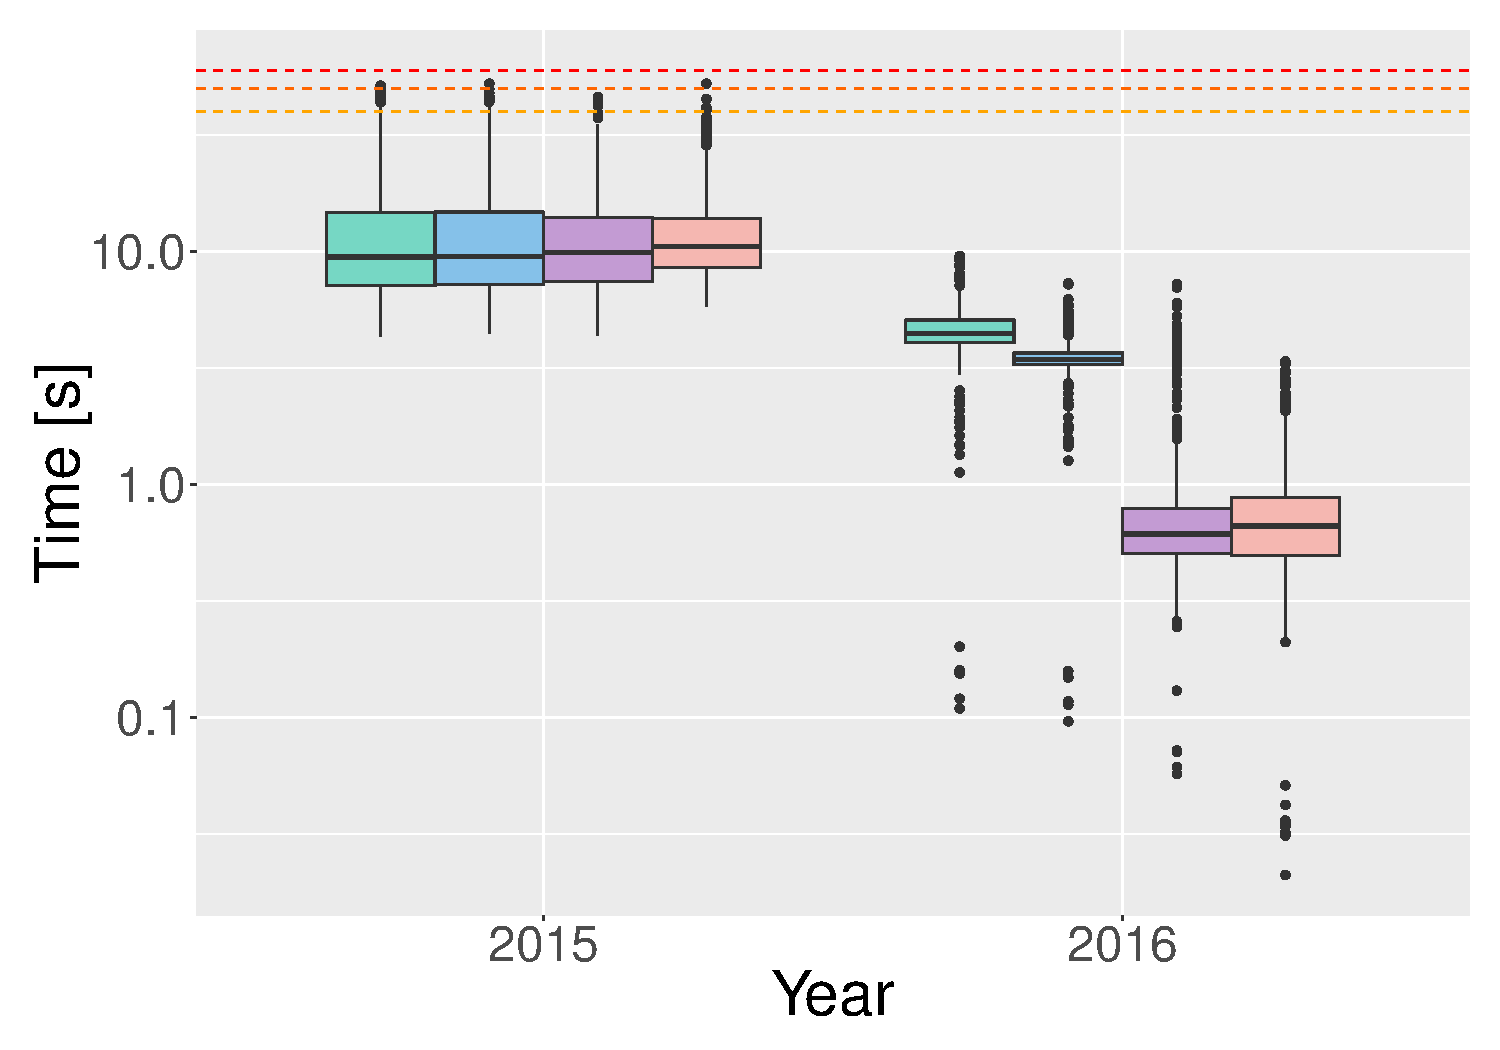
\includegraphics[width=0.45\textwidth]{liveqa-actual.pdf}
\caption{Response times compared to the $4$ systems fielded by
RMIT in 2015.
Clearly, the improved early stage performance provides a much larger
budget for late-stage processing.
The yellow, orange and red horizontal lines denote the $40$, $50$ and
$60$ second intervals respectively, where performance begins to
affect the likelihood that results will be returned within the time
budget.}
\label{fig:2016-times}
\end{figure}


\begin{figure}[t]
\centering
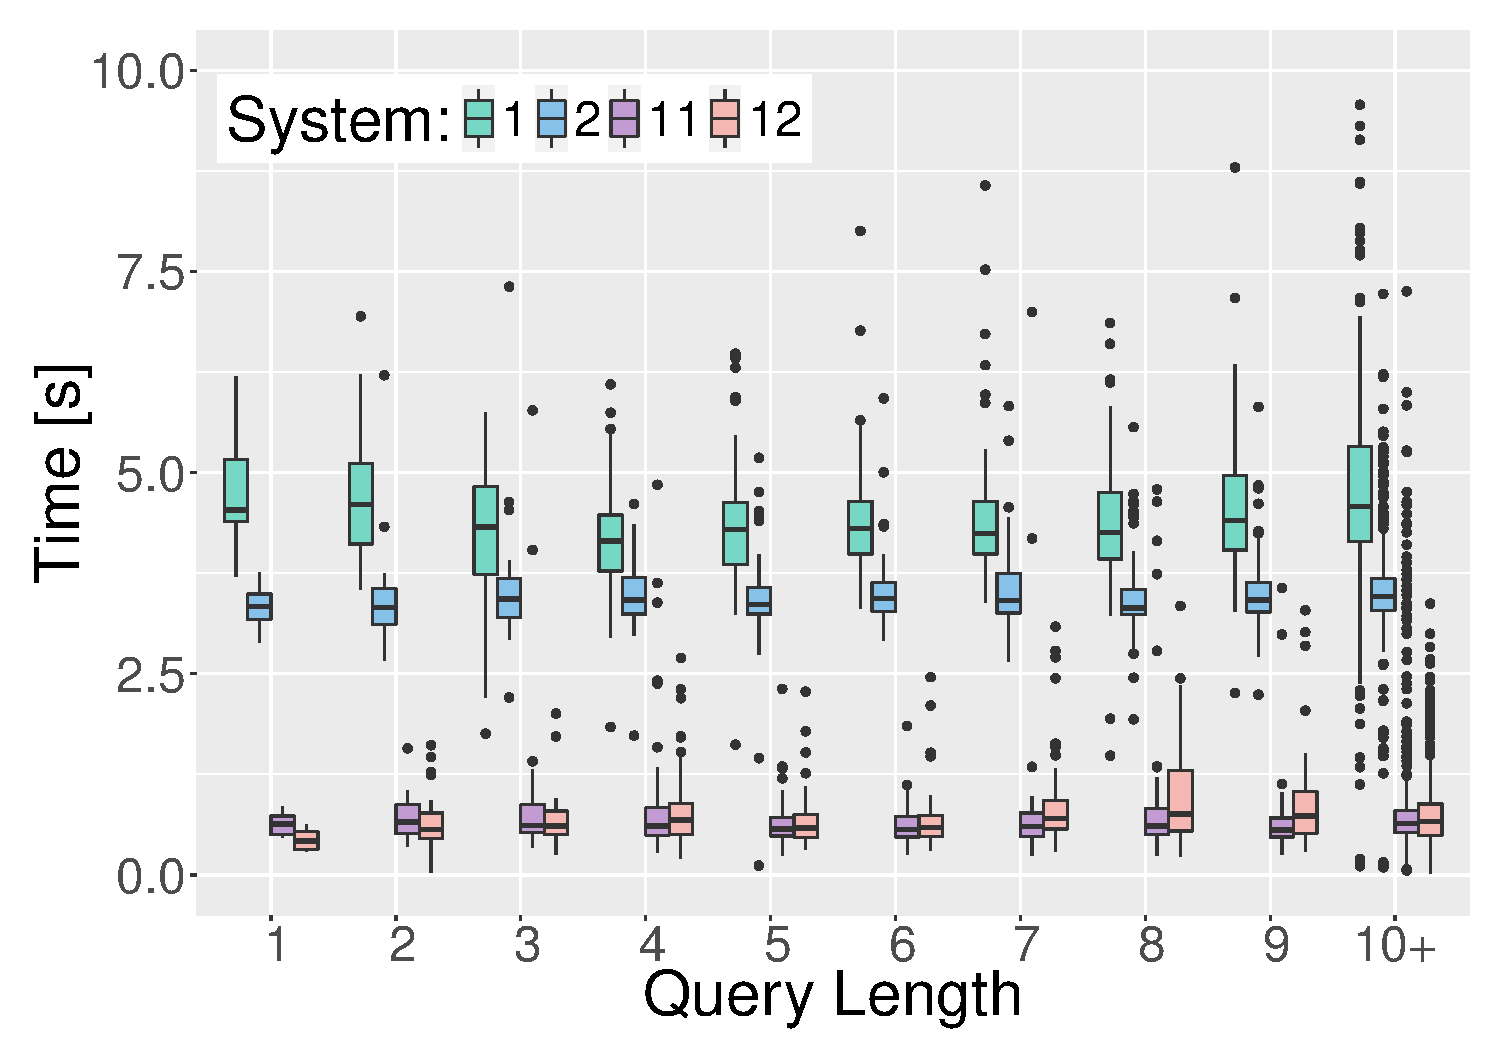
\includegraphics[width=0.45\textwidth]{liveqa-actual-len.pdf}
\caption{Response times broken down by query length for all $4$
systems used in the challenge.
Query length does not adversely effect the timings, as these
are likely dominated by the second-stage summarization module.}
\label{fig:2016-lens}
\end{figure}


\section{Conclusion}

We have explored four different system configurations for the TREC
LIVEQA Track in 2016.
While we remain pleasantly surprised with the performance of our
simple system configurations, we are hopeful that further improvements 
can still be realized through better filtering steps, better query
parsing and prediction, and increasing the coverage in our current
documents collections.

In summary, we found that retrieving the top-$k$ paragraphs from a
local test collection combined with generating a succinct summary of
these paragraphs provided the most effective solution.
Additionally, we show that the first-stage retrieval efficiency cost
is dominated by the second-stage re-ranking/summarizing stage.
Finally, we show large efficiency improvements compared to our
systems from the 2015 LiveQA challenge, which allows us to include
more expensive stages in future work.
%We hope that further post-run analysis will provide insight into why
%the approaches were not successful in our current system
%configurations.

\myparagraph{Acknowledgment}

This work was supported in part by the Australian Research Council's
{\emph{Discovery Projects}} Scheme (DP140102655).
Shane Culpepper is the recipient of an Australian Research Council
DECRA Research Fellowship (DE140100275).
The statements made herein are solely the responsibility of the
authors.


%\bibliographystyle{IEEEtran} 
\balance
\bibliographystyle{plainnat} 
\bibliography{p}

\end{document}

